\documentclass[11pt]{article}
\usepackage[scaled=0.92]{helvet}
\usepackage{geometry}
\geometry{letterpaper,tmargin=1in,bmargin=1in,lmargin=1in,rmargin=1in}
\usepackage[parfill]{parskip} % Activate to begin paragraphs with an empty line rather than an indent %\usepackage{graphicx}
\usepackage{amsmath,amssymb, mathrsfs, dsfont}
\usepackage{mathtools}

\usepackage{tabularx}
\usepackage[font=footnotesize,labelfont=bf]{caption}
\usepackage{graphicx}
\usepackage{xcolor}
%\usepackage[linkbordercolor ={1 1 1} ]{hyperref}
%\usepackage[sf]{titlesec}
\usepackage{natbib}
\usepackage{../../Tianpei_Report}

%\usepackage{appendix}
%\usepackage{algorithm}
%\usepackage{algorithmic}

%\renewcommand{\algorithmicrequire}{\textbf{Input:}}
%\renewcommand{\algorithmicensure}{\textbf{Output:}}



\begin{document}
\title{Lecture 9: Control with Function Approximation}
\author{Tianpei Xie}
\date{ Aug 12th., 2022 }
\maketitle
\tableofcontents
\newpage
\section{Introduction}
Recall that in Tabular methods, the control problem is solved by estimation of action-value fucntion $q_{\pi}(s, a)$. We have on-policy and off-policy control updates:
\begin{align*}
Q(S_{t}, A_{t}) &\leftarrow Q(S_{t}, A_{t}) + \alpha_{t}\brac{\hat{G}_{t}  - Q(S_{t}, A_{t})}.  \\
 \text{  \textbf{Sarsa} }\quad\hat{G}_{t} &= R_{t+1} + \gamma Q(S_{t+1}, A_{t+1}) \\
\text{  \textbf{Q-Learning} }\quad\hat{G}_{t} &=  R_{t+1} + \gamma \max_{a'\in \cA(S_{t+1})}Q(S_{t+1}, a')  \\
 \text{  \textbf{Expected Sarsa} }\quad\hat{G}_{t} &= R_{t+1} + \gamma\sum_{a'}\pi(a'|S_{t+1})Q(S_{t+1}, a') 
\end{align*} Like in on-policy prediction with approximation, we use \textbf{parameterized} function to approximate action-value $q_{\pi}(s, a)\approx \hat{q}(\mb{s}, a, \mb{w})$.

Also recall that when we parameterize the value function in prediction task, the update rule is modified: for instance in TD(0)/Semi-gradient, 
\begin{align*}
\text{(taular method) }V(S_{t}) &\leftarrow V(S_{t}) + \alpha_{t}\paren{R_{t+1} + \gamma V(S_{t+1})  - V(S_{t})} \nonumber\\
\text{(fun. approx.) }\mb{w}_{t+1} &\leftarrow  \mb{w}_{t} + \alpha \brac{R_{t+1} + \gamma \hat{v}(S_{t+1}, \mb{w}_{t}) - \hat{v}(S_{t}, \mb{w}_{t})} \grad{\mb{w}}{\hat{v}(S_{t}, \mb{w}_{t})}
\end{align*} That is, the function $V$ is replaced by its parameter representation $\mb{w}$ and also the \emph{error} term is multiplied by the \emph{gradient} term $\grad{\mb{w}}{\hat{v}(S_{t}, \mb{w}_{t})}$. We can see that after the similar modification, the control updates can still be applied. 

\section{Episodic Semi-gradient Control}
\begin{figure}
\begin{minipage}[t]{1\linewidth}
  \centering
  \centerline{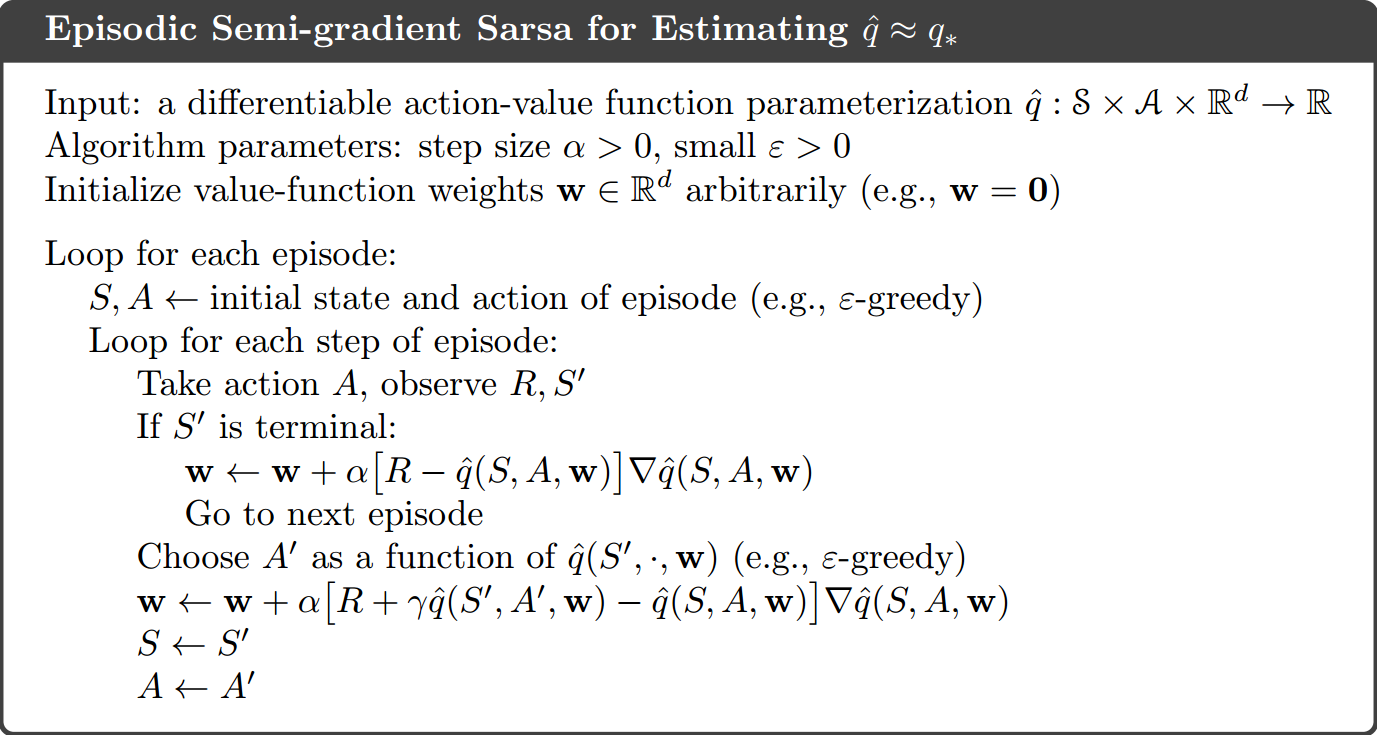
\includegraphics[scale = 0.3]{semi_grad_sarsa.png}}
\end{minipage}
\caption{\footnotesize{\textbf{The episodic semi-gradient Sarsa}}}
\label{fig: semi_grad_sarsa}
\end{figure}
Based on similar derivation and using Tabular Sarsa as reference, we have the following control updates under action-value function approximation $\hat{q}(\mb{s}, a, \mb{w})$: 
\begin{align}
\text{(SGD) } \mb{w}_{t+1} &\leftarrow  \mb{w}_{t} + \alpha \brac{\hat{G}_{t} - \hat{q}(S_{t}, A_{t}, \mb{w}_{t})}\grad{\mb{w}}{\hat{q}(S_{t}, A_{t}, \mb{w}_{t})} \label{eqn: sgd_q}\\
\text{(\textbf{semi-gradient (SARSA)}) }&\nonumber\\
\mb{w}_{t+1} &\leftarrow  \mb{w}_{t} + \alpha \brac{R_{t+1} + \gamma \hat{q}(S_{t+1}, A_{t+1}, \mb{w}_{t}) - \hat{q}(S_{t}, A_{t}, \mb{w}_{t})} \grad{\mb{w}}{\hat{q}(S_{t}, A_{t}, \mb{w}_{t})}  \label{eqn: semi_grad_td_q}
\end{align} We call this method in  \eqref{eqn: semi_grad_td_q} \emph{\textbf{episodic semi-gradient one-step Sarsa}}. In SGD \eqref{eqn: sgd_q}, we assume that we have access to a set of input-output pairs $((S_{t}, A_{t}), \hat{G}_{t})$, where input is the sample state-action pair $(S_{t}, A_{t})$. In semi-gradient, the output is replaced by reward plus previous estimates $R_{t+1} + \gamma \hat{q}(S_{t+1}, A_{t+1}, \mb{w}_{t})$.  For a constant policy, this method converges in the same way that TD(0) does, with the same kind of error bound.

To form control methods, we need to couple such action-value prediction methods with techniques for policy improvement and action selection. For large continuous actions, or to actions from large discrete sets, this is a challenging task and an ongoing research topic. For action set that is \textbf{discrete} and \textbf{not too large}, we can use $\epsilon$-greedy algorithm to find the optimal action $A_{t}^{*} = \argmax_{a} \hat{q}(S_{t}, a, \mb{w}_{t})$ with probability $1-\epsilon$.  Figure \ref{fig: semi_grad_sarsa} shows the episodic semi-gradient SARSA for on-policy control. This is essentially the same as Tabular SARSA except that replacing the value function updates with the updates on its parameters. 

Similar to SARSA, we can construct the update rule for off-policy \textbf{Q-learning} and \textbf{Expected SARSA} for function approximation based on its tabular form:
\begin{align}
\mb{w}_{t+1} &\leftarrow  \mb{w}_{t} + \alpha\, \delta_{t}\,\grad{\mb{w}}{\hat{q}(S_{t}, A_{t}, \mb{w}_{t})}  \nonumber\\
\text{  \textbf{Q-Learning} }\quad \delta_{t}&:=\brac{R_{t+1} + \gamma \max_{a'}\hat{q}(S_{t+1}, a', \mb{w}_{t}) - \hat{q}(S_{t}, A_{t}, \mb{w}_{t})}   \label{eqn: semi_grad_q_learning}\\
 \text{  \textbf{Expected Sarsa} }\quad \delta_{t} &= \brac{R_{t+1} +\gamma\sum_{a'}\pi(a'|S_{t+1})\hat{q}(S_{t+1}, a', \mb{w}_{t}) - \hat{q}(S_{t}, A_{t}, \mb{w}_{t})}  \label{eqn: semi_grad_exp_sarsa} 
\end{align} Similar to SARSA, these algorithms apply to discrete and small action space, since it requires a complete scan of all possible actions at given state. Replacing \eqref{eqn: semi_grad_td_q} with \eqref{eqn: semi_grad_q_learning} or \eqref{eqn: semi_grad_exp_sarsa} in Figure \ref{fig: semi_grad_sarsa}, we have complete description of \textbf{semi-gradient off-control Q-learning} and \textbf{Expected SARSA}.   

Like prediction task, we can use deep neural network to estimate the action-value function $Q$ such as Deep Q-Network. For more discussion on Deep RL, see in \citep{franccois2018introduction}


\section{Average Rewards as New Problem Setting for Continuing Tasks}
\begin{figure}
\begin{minipage}[t]{1\linewidth}
  \centering
  \centerline{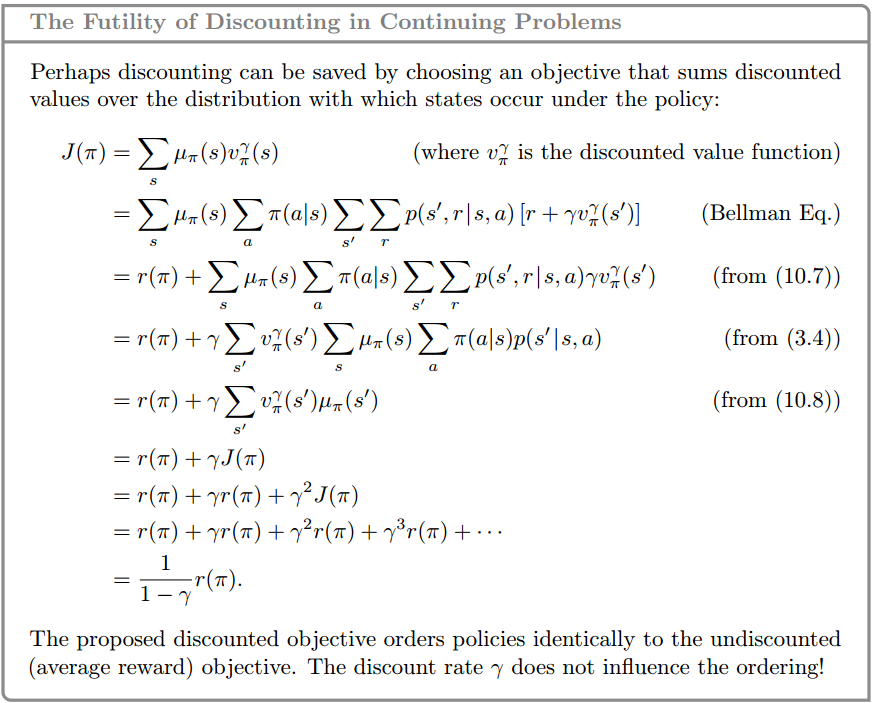
\includegraphics[scale = 0.45]{discount_count_problem.png}}
\end{minipage}
\caption{\footnotesize{\textbf{Use of discount factor in continuing task is futile}}}
\label{fig: discount_count_problem}
\end{figure}
The goal for reinforcement learning is to maximize the cumulative rewards or returns. By far, our definitions of returns in episodic tasks and continuing tasks are focusing on cumulation i.e. summation. This section, we introduce a new concept for continuing task, the average rewards.
\begin{itemize}
\item \textbf{Returns for episodic task}: In episodic task, the task is terminated at some time $T$. The return is a finite number
\begin{align}
G_{t} &= \sum_{\tau=0}^{T-t-1}R_{\tau+t+1} < \infty \label{eqn: returns_episodic}
\end{align}

\item \textbf{Discounted returns for continuing task}: In continuing task, there is no termination and the natural sum is infinite thus improper. In order to obtain finite return, we need to add discount factor $\gamma \in [0, 1)$
\begin{align}
G_{t} &= \sum_{\tau=0}^{\infty}\gamma^{\tau} R_{\tau+t+1} < \infty \label{eqn: returns_discount_continuing}
\end{align} Note that the choice of $\gamma$ has significant impact on the behavior of learning agents. When $\gamma \rightarrow 1$, the agent emphasize the long-term gain over shot-term gain. When $\gamma \rightarrow 0$, it does the opposite.  

Unlike the tabular cases, in which the returns from each state can be separately identified and averaged, using the discounted returns for function approximation in counting tasks is \textbf{questionable}, esp. when the MDP is ergodic and has become \textbf{stationary} in the long run. 

Consider an infinite sequence of returns with no beginning or end, and no clearly identified states. The states might be represented only by feature vectors, which
may do little to distinguish the states from each other. As a special case, \emph{all of the feature vectors may be the same}. Thus one really has only the \textbf{reward sequence} (and the actions), and performance has to be assessed purely from these. In particular, the \emph{ordering} of all policies in the average discounted return setting
would be exactly \textbf{the same} as in the \emph{average-reward} setting. When the MDP for contining task reach to \textbf{steady state} (i.e. the maginal distribution of each state is not changing over time), due to transition-symmetry, \textbf{each time step is exactly the same as every other}. You cannot tell where it is since there is no beginning and no end for a sequence of returns $(\ldots, G_{t}, G_{t+1}, \ldots)$.  With discounting, every reward will appear exactly once in each position in some return. (i.e. $R_{t}$ appears in every $G_{t-1}, G_{t-2}, \ldots, $). The weight on the $t$-th reward is thus $\sum_{\tau=0}^{\infty}\gamma^{\tau} = \frac{1}{1-\gamma}$.

In fact, we can show that in ergodic continuing task, because all states are the same, they are all weighted by this, and thus the \emph{average} of the returns will be the asympototic discount factor $\frac{1}{1-\gamma}$ times the \textbf{average reward}, or $r(\pi)/(1-\gamma)$.  Figure \ref{fig: discount_count_problem} shows a proof of this. 

The root cause of the difficulties with the \textbf{discounted control} setting is that with \underline{\textbf{function}} \underline{\textbf{approximation}} we have \underline{\textbf{lost the \emph{policy improvement theorem}}}. It is no longer true that if we change the policy to improve the discounted value of one state then we are guaranteed to have improved the overall policy in any useful sense. In fact, the lack of a policy improvement theorem is also a theoretical lacuna for the total-episodic and average-reward settings. Once we introduce function approximation we can no longer guarantee improvement for any setting.



\item \textbf{Average reward and Differential returns for continuing task}: Unlike discounted returns, average reward \textbf{does not} have \emph{discount factor} $\gamma$. In the average-reward setting, the quality of a policy $\pi$ is defined as the \emph{\textbf{average rate} of \textbf{reward}}, or simply \textbf{average reward}, while following that policy, which we denote as $r(\pi)$:
\begin{align}
r(\pi) &= \lim_{T\rightarrow \infty}\frac{1}{T}\E{\pi}{G_{0:T} \big| S_{0}, A_{0:t-1} \sim \pi} \nonumber\\
 &=\lim_{T\rightarrow \infty}\frac{1}{T}\sum_{t=0}^{T}\E{\pi}{R_{t} \big| S_{0}, A_{0:t-1} \sim \pi}  \label{eqn: avg_reward_discount_continuing}\\
&= \lim_{t\rightarrow \infty}\E{\pi}{R_{t} \big| S_{0}, A_{0:t-1} \sim \pi}  \label{eqn: avg_reward_discount_continuing2}\\
&= \sum_{s}\mu_{\pi}(s)\sum_{a}\pi(a|s) \sum_{s', r}p(s', r| s, a)r,  \label{eqn: avg_reward_discount_continuing3}
\end{align}  where the expectations are conditioned on the initial state, $S_0$, and on the subsequent actions, $A_0, A_1, \ldots, A_{t-1}$, being taken according to $\pi$. $\mu_{\pi}(s)$ is the \underline{\textbf{steady-state distribution}}. $$\mu_{\pi}(s) = \lim_{t\rightarrow \infty} \text{Pr}\{S_t =s |A_{0:t-1} \sim \pi\},$$ which is assumed to exist for any $\pi$ and to be \textbf{independent} of $S_0$. This assumption about the MDP is known as \underline{\textbf{ergodicity}}  In other words, it relies on there being a long term stable distribution of states under any particular policy. The defintion of average rewards for continuing tasks can only be applied when the underling MDP is \textbf{ergodic}.  From \eqref{eqn: avg_reward_discount_continuing2} we can see that \textbf{the average reward is the reward obtained at when MDP reaches the stationary state}.

We consider $\pi_{*} = \argmax_{\pi}r(\pi)$ as the \textbf{optimal policy}, which is the basis for \textbf{policy-based learning} algorithm. 

Moreover, according to MDP, the stationary distribution is the \textbf{fixed-point solution} the equation below:
\begin{align}
\mu_{\pi}(s') &= \sum_{s}\mu_{\pi}(s)\paren{\sum_{a}\pi(a|s) \sum_{s'}p(s'| s, a)} \label{eqn: stationary_dist_eqn}
\end{align} 

With the average rewards, we can define the the \textbf{differential return} as the cumulative \emph{difference} between rewards and the average reward:
\begin{align}
G_{t} &= \sum_{\tau=0}^{\infty}\paren{R_{\tau+t+1} - r(\pi)} < \infty \label{eqn: returns_diff_continuing}
\end{align}  Replacing \eqref{eqn: returns_discount_continuing} or \eqref{eqn: returns_episodic} with \eqref{eqn: returns_diff_continuing}, we can obtain the definition of \textbf{\emph{differential value function}} of expected differential returns given state or state-action pair: $v_{\pi}(s):= \E{\pi}{G_{t}  | S_{t}=s}$ and $q_{\pi}(s, a):= \E{\pi}{G_{t}  | S_{t}=s, A_{t}=a}$.  The differential returns measures how well our policy behaves as compared to the average reward under a \textbf{fixed policy}. We can also reformulate the \textbf{Bellman equation} and \textbf{Bellman optimality equation} for \textbf{average reward MDP} by removing $\gamma$ and replacing reward $r$ with differential reward $r-r(\pi)$: 
\begin{align}
v_{\pi}(s) &= \sum_{a}\pi(a|s)\sum_{s', r}p(s', r| s, a)\brac{r - r(\pi) + v_{\pi}(s')}, \quad \forall\,\; s\in \cS \label{eqn: bellman_eqn_value_diff} \\
&= \E{\pi}{R_{t+1} - r(\pi)  + \,v_{\pi}(S_{t+1}) | S_{t} = s} \label{eqn: bellman_eqn_value_diff_2}\\
q_{\pi}(s, a) &=\sum_{s', r}p(s', r|s,a)\brac{r - r(\pi) +  \sum_{a'}\pi(a'|s')q_{\pi}(s', a')} \quad \forall\,\; s\in \cS, \; a\in \cA(s) \label{eqn: bellman_eqn_value_action_diff}\\
&=\E{\pi}{R_{t+1} - r(\pi)  + q_{\pi}(S_{t+1}, A_{t+1}) | S_{t}=s, A_{t}=a}  \label{eqn: bellman_eqn_value_action_diff_2}\\
v_{*}(s) &= \max_{a\in \cA(s)}\sum_{s', r}p(s', r|s, a)\brac{r - \max_{\pi}r(\pi) + v_{*}(s')} \label{eqn: bellman_opt_eqn_value_diff}\\
 &=  \max_{a\in \cA(s)}\E{}{R_{t+1} - \max_{\pi}r(\pi) + v_{*}(S_{t+1}) | S_{t}=s, A_{t}=a} \label{eqn: bellman_opt_eqn_value_diff_2} \\
 q_{*}(s, a) &=\sum_{s'}\sum_{r}p(s', r|s, a)\brac{r  - \max_{\pi}r(\pi) +  \max_{a'\in \cA(s)}q_{*}(s', a')}  \label{eqn: bellman_opt_eqn_value_action_diff}\\
 &=  \E{}{R_{t+1}  - \max_{\pi}r(\pi)+ \max_{a'\in \cA(s)}q_{*}(S_{t+1}, a') \Big| S_{t}=s, A_{t}=a} \label{eqn: bellman_opt_eqn_value_action_diff_2}
\end{align} Note that in Bellman optimality equation for differential returns, we also need to choose \textbf{optimal average rewards} $\max_{\pi}r(\pi)$ instead of using average reward itself since the optimal value function is not a function of policy $\pi$.
\begin{figure}
\begin{minipage}[t]{1\linewidth}
  \centering
  \centerline{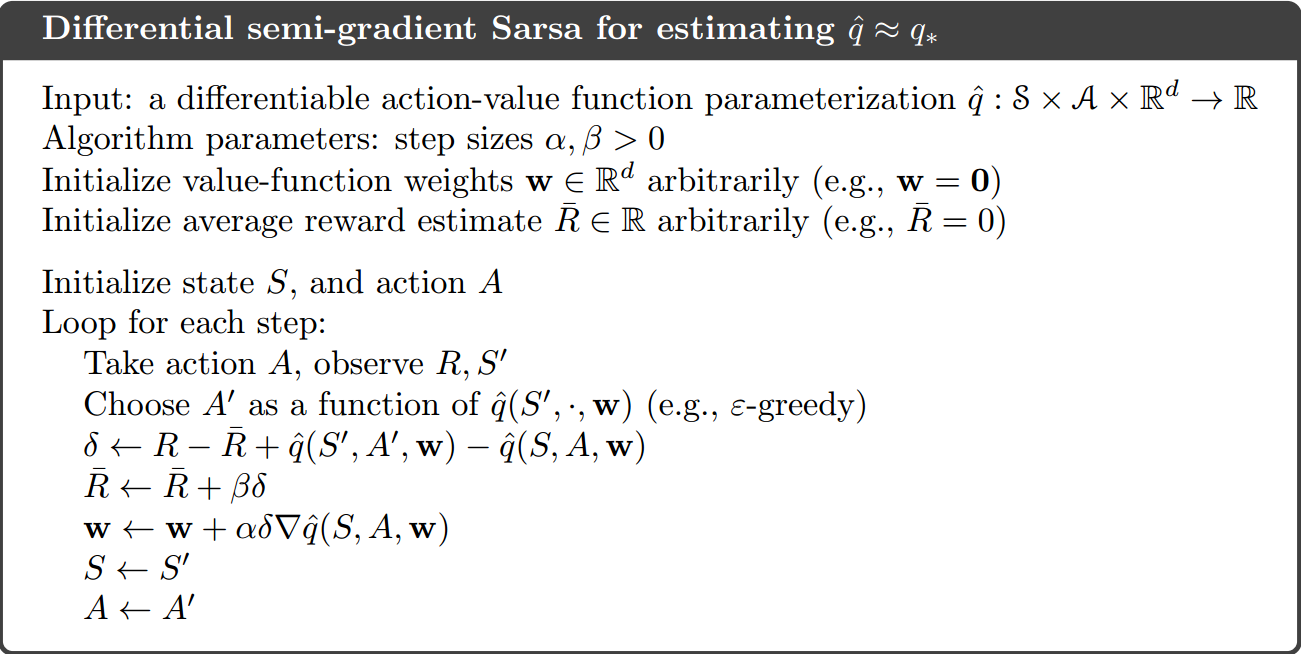
\includegraphics[scale = 0.3]{semi_grad_sarsa_diff.png}}
\end{minipage}
\caption{\footnotesize{\textbf{Differential semi-gradient SARSA }}}
\label{fig: semi_grad_sarsa_diff}
\end{figure}
Based on these Bellman equations, we can derive the \textbf{\emph{Differential TD error}} for differential returns:
\begin{align}
\text{  \textbf{Sarsa} }\quad\delta_{t} &= R_{t+1} -  \bar{R}_{t}  +  Q(S_{t+1}, A_{t+1}) -  Q(S_{t}, A_{t}) \label{eqn: sarsa_diff}\\
\text{  \textbf{Q-Learning} }\quad\delta_{t} &=  R_{t+1}  -  \bar{R}_{t}  +  \max_{a'\in \cA(S_{t+1})}Q(S_{t+1}, a') -  Q(S_{t}, A_{t})  \label{eqn: q_learn_diff} \\
 \text{  \textbf{Expected Sarsa} }\quad\delta_{t} &= R_{t+1}  -  \bar{R}_{t}  + \sum_{a'}\pi(a'|S_{t+1})Q(S_{t+1}, a') -  Q(S_{t}, A_{t})  \label{eqn: expected_sarsa_diff}
\end{align} Note that instead of computing $r(\pi)$ which requires knowledge of model $p(s'|s, a)$, we use the sample average reward $\bar{R}_{t}$ as estimate, which is updated by accumulation of TD error $\bar{R}_{t+1} = \bar{R}_{t} + \beta\,\delta_{t} = \beta\sum_{t}\delta_{t}$. Figure \ref{fig: semi_grad_sarsa_diff} shows the \textbf{differential semi-gradient SARSA}.
\end{itemize}

\newpage
\begin{exercise} Proof of Bellman equation \eqref{eqn: bellman_eqn_value_diff_2} for average rewards MDP. 
\end{exercise}
\begin{solution}
\begin{align*}
v_{\pi}(s) &=\E{\pi}{G_{t}|S_{t}=s}\\
&= \E{\pi}{\sum_{\tau=t+1}^{\infty}\paren{R_{\tau} - r(\pi)} \Big| S_{t}=s} \\
&=  \E{\pi}{R_{t+1} - r(\pi) + \sum_{\tau=t+2}^{\infty}\paren{R_{\tau} - r(\pi)} \Big| S_{t}=s} \\
&= \E{}{\E{\pi}{R_{t+1} - r(\pi) + \sum_{\tau=t+2}^{\infty}\paren{R_{\tau} - r(\pi)} \Big| S_{t+1}, S_{t}=s}\Big| S_{t}=s}\\
&= \E{}{\E{\pi}{R_{t+1} - r(\pi) + G_{t+1} \Big| S_{t+1}, S_{t}=s}\Big| S_{t}=s}\\
&(\text{constant since policy fixed})\\
&= \E{}{R_{t+1} - r(\pi) + \E{\pi}{G_{t+1} \Big| S_{t+1}, S_{t}=s}\Big|  S_{t}=s}\\
&(\text{by Markov Property})\\
&= \E{}{R_{t+1} - r(\pi) + \E{\pi}{G_{t+1} \Big| S_{t+1}}\Big|  S_{t}=s}\\
&=  \E{}{R_{t+1} - r(\pi) + v_{\pi}(S_{t+1})\Big|  S_{t}=s}. \quad \QEDA
\end{align*} 
\end{solution}


\begin{exercise} Proof of Bellman optimality equation \eqref{eqn: bellman_opt_eqn_value_diff_2} for average rewards MDP. 
\end{exercise}
\begin{solution}
\begin{align*}
v_{*}(s) &:= \max_{a\in \cA(s)}\max_{\pi}\E{\pi}{G_{t}|S_{t}=s, A_{t} = a}\\
&=\max_{a\in \cA(s)}q_{\pi_{*}}(s, a)\\
&(\text{the optimal policy }\pi_{*}=\argmax_{\pi}\E{\pi}{G_{t}|S_{t}}\text{ is chosen}) \\
&=\max_{a\in \cA(s)}\E{\pi}{\sum_{\tau=t+1}^{\infty}\paren{R_{\tau} - r(\pi_{*})} \Big| S_{t}=s, A_{t} = a}\\
&=\max_{a\in \cA(s)}\E{\pi}{R_{t+1} - r(\pi_{*}) + \sum_{\tau=t+2}^{\infty}\paren{R_{\tau} - r(\pi_{*})} \Big| S_{t}=s, A_{t} = a}\\
&= \max_{a\in \cA(s)}\E{\pi}{\E{}{R_{t+1} - r(\pi_{*}) + \sum_{\tau=t+2}^{\infty}\paren{R_{\tau} -r(\pi_{*})}\Big| S_{t+1}, S_{t}=s, A_{t} = a}  \Big| S_{t}=s, A_{t} = a}\\
&= \max_{a\in \cA(s)}\E{}{R_{t+1} - r(\pi_{*}) + \E{\pi}{\sum_{\tau=t+2}^{\infty}\paren{R_{\tau} - r(\pi_{*})}\Big| S_{t+1}}  \Big| S_{t}=s, A_{t} = a}\\
&= \max_{a\in \cA(s)}\E{}{R_{t+1} - r(\pi_{*}) + \max_{\pi}\E{\pi}{G_{t+1}|S_{t+1}}  \Big| S_{t}=s, A_{t} = a}\\
&(\text{the optimal policy }\pi_{*}=\argmax_{\pi}\E{\pi}{G_{t+1}|S_{t+1}} = \argmax_{\pi}r(\pi)) \\
&=\max_{a\in \cA(s)}\E{}{R_{t+1} - \max_{\pi}r(\pi) + v_{*}(S_{t+1})  \Big| S_{t}=s, A_{t} = a}. \quad \QEDA
\end{align*} 
\end{solution}
%
\newpage
\bibliographystyle{plainnat}
\bibliography{reference.bib}
\end{document}